\section{Software-to-Hardware Allocation Problem}\label{sec_problem}
The software applications are allocated on the execution platform by mapping the software-component replicas (or software components)  \ttsss{Q} to the computing units $\mathcal{N}$. The software-to-hardware allocation problem is to find the mapping $\x:\sss{Q}\rightarrow\mathcal{N}$ that satisfies the user-defined requirements of the software applications, but also minimize the total power consumption of the applications, where $\textbf{x}$ is a possible mapping matrix, and {\ttxkij } represents the mapping of the software component \ttsss{q}[k][i,j] to the compuing unit $n_h$, where $h=\xkij$, of the application $A_k$.

\subsection{Total Power Consumption}
The total power consumption of the applications $\mathcal{P}_{total}(\x)$ is computed as the sum of the power consumption of the computing units to which the applications are allocated. The power consumption of a unit is computed according to the linear model proposed by Fan et al. \cite{Fan2007PowerComputer} as shown by Equation~(\ref{eqn_powerconsumption}), which is directly proportional to its load (or utilization) and is inductively formulated from experimental results.
\begin{equation}
\label{eqn_powerconsumption}
\mathcal{P}(u)=P_{idle} + (P_{busy}-P_{idle})*u,
\end{equation}
where $u$ is the utilization of a computing unit, $P_{idle}$ and $P_{busy}$, respectively refer to the power consumption measured at minimum and maximum processor load. The parameters of the model can be obtained by running performance benchmark suits, e.g., MiBench \cite{Guthaus2001MiBench:Suite}, AutoBench \cite{EMBC2018AutoBenchProcessors}, etc. 

The utilization of a computing unit is computed as a sum of the utilization of the tasks mapped to it $\ssb{T}[n_h]$, which are identified by traversing the mapping elements-wise \ttxkij{} as shown in Equation~(\ref{eqn_tasks_per_node}), where $\ssb{T}$ refers to the tasks implementing the component type $\sss{c}$.
\begin{align}
\label{eqn_tasks_per_node}
\ssb{T}[n_h]=\{\sss{T} | \forall kij\ h=\xkij \}   \mbox{  forall } h= 1,...,n_N
\end{align}

Then, the utilization of the units, indicated by the vector $(u_1,...,u_{n_N})$, is 
\[
	(u_1,...,u_{n_N})(\x)=\sum_{\tau\in \ssb{T}[n_h]}{\mathcal{U}(\tau,n_h), \mbox{ for all } h=1,..,n_{N}},
\] where $\mathcal{U}(\tau,n)=WCET_{\tau,n}/P_\tau$ computes utilization of the task $\tau$ on the unit $n$. Thus, the total power consumption of the applications is formulated as
\begin{align}
\label{eqn_total_power}
\mathcal{P}_{total}(\textbf{x})  = \sum_{h=1}^{n_N}{\mathcal{P}(u_h(\x))} \mbox{ for all } h=1,..,n_{N},  
\end{align}

\subsection{Tasks  and Messages Timing Constraints}
The tasks timing constraints ensure that the tasks in the distributed system meet their respective deadlines, that is 
$\forall \tau\in \ssb{T}[n_h] \ ResponseTime_\tau(\x)\leq Deadline_\tau$ for all $h=1,...,n_N$, following Equation~(\ref{eqn_tasks_per_node}). Similarly, the messages timing constraints ensure that the response-time of message in the CAN bus meet their respective deadlines. 

The set of messages in the bus is determind by traversing the edges of the tasks graphs. If the edge relates tasks located on different units, a message is used to communicate across the bus, otherwise, no message is used.
%If more than one replica of a task is mapped to a unit, the Tasks replicas mapped to the same unit do not improve realiability of the applications since we assume a permanent failure of computing units would lead to the total failure of the software running on the units. Consequently, the replicas except one are discarded, hence exists only a maximum of one replica per computing unit. The replica can be identified from other replicas based on the unit to which it is mapped. Assume $\tau\in \gr{V}{\at}$ is a task node and $\sss{\mathcal{N}}[k][\tau]$ is the set of units to which its replicas can be mapped. Thus, the replicas of $\tau$ are represented a paired-set $\mathcal{R}=\{(\tau,n)|n\in\sss{\mathcal{N}}[k][\tau]\}$, where $(\tau,n)$ is the replica of $\tau$ mapped to $n$.
%\begin{figure}[h!]
%	\centering
%	\includegraphics[width=0.6\linewidth]{img/task_replication}
%\end{figure}
%To constract the tasks timing constraints, first we arrange the tasks per computing unit, $\ssb{T}[n_h]$, so that the tasks graphs are not traversed everytime the response-time of tasks is computed. So, after traversing the tasks graphs, consequently in each task node $\tau\in V(\at(\x))$, we check if the replica $\tau_{i,j}$ is mapped to $n_h\in N$. If the condition is true, we collect the task node $\tau_i$ as shown in Equation (\ref{eqn_tasks_nodes}). 
%\begin{align}
%\label{eqn_tasks_nodes}
%T_{n_h}&=\{\tau\in \mathcal{V}(\at(\x)) | \forall j\in\sss{\mathcal{N}}[k][\tau_i][b]\ j=n_h\} & \mbox{ for all } h=1,...,n_N,
%\end{align}
%where $\mbox{ where }h=\xkij$. The complexity of this equation, considering an adjucency matrix implementation, is exponential time $O(\sum{|\gr{V}{\at}|*n_N^2})$, where $\gr{V}{\at}$ is tasks nodes in $\at$, and $N$ is the total computing units in the distributed system. 
%Subsequently, we calculate the response time of each task $\tau \in T_{m}$ in \ttx by invoking the response-time analyais formula, and construct the tasks timing constraints as shown in Equation (\ref{eqn_tasks_constraints}).
%\begin{align}
%\label{eqn_tasks_constraints}
%\forall \tau\in T_{n} \ ResponseTime_\tau(\x)&\leq Deadline_\tau
%\end{align}
%\subsubsection{Messages Timing Constraints}
%The messages timing constraints ensure that the response-time of message in the CAN bus meet their respective deadlines, which is equal to their periods. The messages $M$ in \ttx are determined from the communication links of the tasks graphs. Assume $(t1,t2)\in\gr{E}{\at}$ is a link in the task graph. 
However, due to replication, the edge may represent a set of subedges, where each subedge relates tasks replicas on both sides of the edge. Consider $\sss{\mathcal{R}}[k][\tau][b]=\{(\tau,n)\in\tau\times\sss{N}[k][\tau]\}$ is the set of the replicas of type $\tau\in\gr{V}{\at}$, now assume $(t1,t2)\in\gr{E}{\at}$ is an edge in the task graph and  $\sss{\mathcal{R}}[k][t2][b], \sss{\mathcal{R}}[k][t2][b]$ are the replicas of type $t1$ and $t2$, respectively. The set of subedges between $t1$ and $t2$ $\sss{\mathcal{R}}[k][t2][b]\times\sss{\mathcal{R}}[k][t2][b]$, and the set of messages in these subedges are where the latter relates tasks replicas located on different nodes. By extension, the set of message in the bus i$M$ determined as,
\begin{equation}
\label{eqn_tasks_nodes}
M=\{m_{i,j} | \forall (t1,t2)\in \mathcal{E}(\atx)\forall (i,j)\in\sss{\mathcal{R}}[k][t1][b]\times\sss{\mathcal{R}}[k][t2][b]\ n_i\neq n_j\},
\end{equation}
where $(i,j)$ is a sub-link of $(t1,t2)$, $m_{ij}$ is the message that the replica $i$ uses to communicate with the replica $j$, $n_i,n_j\in \mathcal{N}$.  

We assume the messages inherit the timing and criticality specifications of the sending tasks, thus $P_{m_i }= P_{t1}$, $\mathrm{CL}_{m_i}=\mathrm{CL}_{t1}$.% so that the criticality is preserved at the network, as well. Thus, messages constrains are $\forall m\in M \ ResponseTime_m(\x)\leq Deadline_m$. 

\subsection{End-to-end Timing Constraints}
The end-to-end timing constraints over \ttx ensure that the delays of chains meet thier respective end-to-end requirements, that is $\forall \gamma\in \ssp{\Gamma}\ Delay_\gamma(\x)\leq \sss{\mathrm {EE}}[k][\gamma]$ for all $k=1,...,n_A$. Note: The constrains assumes the tasks and messages constraints are satisfied.

The delay calculation of a chain $\Gamma$ is multiplicity $\Gamma^*$ due to replication. Consdier the chain $\Gamma=(\tau_i)_{i=1}^l=(\tau_1,...,\tau_l)$, then the set of chains with replication is a cartesian product of the tasks replicas (or the tasks nodes mapping to computing units according to $\x$ in the chain, that is $\Gamma^*(\x)= \sss{\mathcal{R}}[k][\tau_1][b]\times,...,\times\sss{\mathcal{R}}[k][\tau_l][b]$, where $l$ is the chain length. Assume we want to calculate the delay of the chain $\gamma\in \Gamma^*$ compositionally, where $\gamma=(t_i)_{i=1}^l=(t_1,...,t_l)$: first we identify the subchains $I$ and messages $J$ of the chain. The subchains $I$ are subsets of the chain $\gamma$ where the communication between the sender and receiver tasks of the chain use a network bus. That is, if $t_i$ is thez sender task, and its receiver task $t_{i+1}$ is mapped to a different unit, i.e., $n_{t_i}\neq n_{t_{i+1}}$, then $(t_h)_{h=i'}^i\in I$ is a subchain of $\gamma$ and $m_{t_i}\in J$ is the message used by the subchain, where $0\leq i'\leq i$, captured by the expression
$
	(I;J)=\{(t_i)_{i=0}^{l-1};m_{t_i} | n_{t_i}\neq n_{t_{i+1}}\}
$.
	
Thus, the delay $\Delta_\gamma(\x)$ for a mapping \ttx is computed as the sum of the age delays of its subchains and the response-times of the messages,
\[
	\Delta_{\gamma}(\x)=\sum_{i\in I_{\gamma}(\x)}{\Delta^{sub}_{i}(\x)} + \sum_{j\in J_{\gamma}(\x)}{[\delta^{msg}_j(\x)+P_{suc(j)}]},
\]
according to the age-delay formula shown in Equation (\ref{eqn_agedelay_multinode}), where $\Delta^{sub}$, $\delta^{msg}$ are the functions that compute the age delay of $i$ subchain, and the response-time of $j$ message, respectively. Thus, the chains timing constraints are formulated over \ttx and applications $A$ using Equation (\ref{eqn_chains_constraints}).
\begin{align}
\label{eqn_chains_constraints}
\forall \gamma \in \ssp{\Gamma} \ \sss{\Delta}[k][{\gamma}](\x) & \leq \sss{\mathrm{EE}}[k][\gamma],
\end{align}
\begin{example}[Delay Calculation] Consider the chain $\Gamma=\tau_1\rightarrow\tau_2\rightarrow\tau_4$ from Figure~\ref{fig_dag_tasks} where $\tau_1$ and $\tau_2$ realize the component types $c_1$, and $\tau_4$ realizes $c_2$. The mapping of the components is shown in Figure~\ref{fig_deployment} (b), i.e., with replication. Thus, the units to which $\tau_1$ and $\tau_2$ are mapped are $\sss{\mathcal{R}}[k][\tau_l][b]=\sss{\mathcal{R}}[k][\tau_2][b]=\{n_1,n_2\}$, and $\tau_4$ to $\sss{\mathcal{R}}[k][\tau_4][b]=\{n_2,n_3\}$, by infering the mappings of respective components. Table~\ref{tbl_chains_with_replication} illustrates how to compute the chains, considering replication of degree 2, which is $\Gamma^* = \sss{\mathcal{R}}[k][\tau_1][b] \times \sss{\mathcal{R}}[k][\tau_2][b] \times \sss{\mathcal{R}}[k][\tau_4][b]$, and also how to compute the subchains and messages of each chain $\gamma\in \Gamma^*$. The delays of the subchains is computed according to the age-delay semantics demonstrated in Subsection~\ref{subsec_cause-effect_chains}.
\end{example} 
\begin{table}[]
	\begin{tabular}{@{}lll@{}}
		\toprule
		$\gamma\in \Gamma^*$ & $i\in I_\gamma$ & $j\in J_\gamma$ \\ \midrule
		$(\tau_1,n_1)\rightarrow (\tau_2,n_1)\rightarrow(\tau_4,n_2)$ & $(\tau_1,n_1)\rightarrow (\tau_2,n_1),(\tau_4,n_2)$ & $m_{(\tau_2,n_1), (\tau_4,n_2)}$ \\
		$(\tau_1,n_1)\rightarrow (\tau_2,n_1)\rightarrow(\tau_4,n_3)$ & $(\tau_1,n_1)\rightarrow (\tau_2,n_1),(\tau_4,n_3)$ & $m_{(\tau_2,n_1), (\tau_4,n_3)}$ \\
		$(\tau_1,n_2)\rightarrow(\tau_2,n_2)\rightarrow(\tau_4,n_2)$ & $(\tau_1,n_2)\rightarrow(\tau_2,n_2)\rightarrow(\tau_4,n_2)$ & $\emptyset$ \\
		$(\tau_1,n_2)\rightarrow(\tau_2,n_2)\rightarrow(\tau_4,n_3)$ & $(\tau_1,n_2)\rightarrow(\tau_2,n_2),(\tau_4,n_3)$ & $m_{(\tau_2,n_2), (\tau_4,n_3)}$ \\ \bottomrule
	\end{tabular}
\caption{Chains-with-Replication of Degree 2 for the Chain $\Gamma=\tau_1\rightarrow\tau_2\rightarrow\tau_4$, its Subchains $I$ and Messages $J$.}
\label{tbl_chains_with_replication}
\end{table}

\subsection{Approximation of Age Delay Calculation}
Due to the replication, the number of chains-with-replication per chain $\Gamma$ grows exponentially as the degree of the replication $D$ linearly increases, $|\Gamma|^D$. Likewise, the length of the chain has a polynomial effect on the number of replicated chains. Moreover, the age-delay calculation is an exhaustive search as demonstrated in Subsection \ref{subsec_cause-effect_chains}. For these main reasons, the age delay computation is expensive especially with replication, which is challenging for metaheuristics, due meta-heuristic algorithms compute large-space candidate solutions. Therefore, we propose an appoximation algorithm to efficiently compute the delays based on worst-case age delay, defined as the maximum delay that be observed in a chain. It is estimated by the following lemma as follows:

\subsection{Approximation of Delay Calculation}\label{subsec_approximation_alg}
Due to the replication, the number of chains-with-replication per chain $\Gamma$ grows exponentially as the degree of the replication $D$ linearly increases, $|\Gamma|^D$. Likewise, the length of the chain has a polynomial effect on the number of replicated chains. Moreover, the age-delay calculation is an exhaustive search as demonstrated in Subsection \ref{subsec_cause-effect_chains}. For these main reasons, the age delay computation is expensive especially with replication as meta-heuristic algorithms compute large-space candidate solutions. Therefore, we propose an approximation algorithm to efficiently compute the delays based on worst-case age delay of a chain mapped to a singe unit.
\begin{lemma}[Worst-case Edge Delay] 
	In the case of replication, the worst-case age delay of a chain mapped to a single computing unit follows the maximization of the age delay formula shown in Equation (), which occurs between the earliest activation of the source task and the latest activation of the sink task plus the maximum worst-case response time of the sink task of a chain. The earliest activation occurs when the source task start time concedes its release time, and latest activation time of the sink task occurs not latter than the second hyper-period since the data is picked up by the source task. 
	
	Thus, the worst-case age delay of a chain mapped to multiple units occur the replicated chain uses the shared network bus the maximum. Therefore, the worst-case edge delay of the chain $\Gamma$ is calculated as follows:
	\begin{align}
		\exists \gamma\in\Gamma^*\ \max{|J_\gamma|}\\
		\Delta^{worst}=2H+\sum_{j\in J_{\gamma}(\x)}{\delta^{msg}_j(\x)}, & \mbox{ where } H=lcm(\gamma)
	\end{align}
\end{lemma}



\subsection{Software-Applications Reliability Constraints}\label{subsec_reliability_constraint}
The applications reliability constraints ensure the mapping $\textbf{x}$ satisfies the user-defined reliability requirements, that is $\forall k\ \rel_{A_k}(\x)\leq RelReq_{A_k}$. 
The reliability of each application is computed over $t$ period of time from the computing units \ttssp{N} and  the shared network bus $B$, where \ttssp{N} hosts \ttar. The reliability is computed assuming exponentially distributed and constant failure rates of the units $\lambda_{n_h}$ as well as the network bus $\lambda_B$. Thus, the reliability of an application is computed as a product of the reliability of the units and the network bus as shown using Equation (\ref{eqn_appreliability_app}). Note: if application does not use the shared  bus $\rel_{B}=1$. Equation (\ref{eqn_nodes_app}) finds the units \ttssp{N} that the application \ttar uses by traversing the partition \ttx in linear time.
\begin{align}
\label{eqn_appreliability_app}
&Reliability_{\ar}(\x)=Reliability_{\ssp{N}}(\x)*Reliability_B\\
\label{eqn_nodes_app}
&\ssp{N}=\{e\in N| \forall ij\ e=m_h\},\mbox{ where } h=\ssx{k}{ij}
\end{align}
Note: we assume applications are mutuallye exclusive, that is no shared components exist between any two applications, therefore, we can safety calculate the reliability of applications independently. Consequently, to increase readability, we remove the superscript $(A_k)$ in the rest of this subsection.

The reliability of the units is $Reliability_N(\x)=e^{-\lambda_N(\x) t}$, where is $\lambda_N(\x)$ is the failure rate of an $N$-unit system over the partition \ttx. The system failure-rate is computed using the state enumeration as shown in \cite{Lucet1999ExactReliability}, which is an exact technique to calculate reliability, as opposed to using series-parallel technique - motivated in Subsection \ref{sub_reliability}. By applying the state enumeration technique, the system failure-rate can be defined as the probability a software application \textit{fails} in the probability space $\langle \Omega,\xi,p,f\rangle$.
\begin{itemize}
	\item $\Omega=\{0,1\}$ are the possible outcomes (or states) of a computing unit. Assume the Boolean variable $s_h\rightarrow\Omega$, which indicates the state of $n_h$, then $s_h=0$ indicates $n_h$ fails and $s_h=0$ indicates $n_h$ operates. Thus, for computing units $N=\{n_1,..,n_{n_N}\}$, the states of the units (or configuration) is indicated by the $N$-cardinality set $S=\{s_1,...,s_{n_N}\}$.
	
	\item $\xi=\Omega^S$ are elementary events that correspond to the possible configurations of the units $N$, therefore, the events are mutually exclusive. Consider $N=\{n_1,n_2,n_3\}$, Table (\ref{tbl_application_rel}) shows the their possible configurations $\xi$. Assume the configuration $s\in \xi=\{0,1,0\}$, it shows $n_1$ and $n_3$ fail as indicated by $s_1=0,s_3=0$, respectively, and $n_2$ operates as indicated by $s_2=1$. 
	
	\item $p:\xi\rightarrow[0,1]$ assings the configurations probabilities using
	\[\forall s\in \xi\  p_s=\prod_{h=1}^{n_N}{\lambda_{n_h}*(1-s_h)+(1-\lambda_{n_h})*s_h}\]
	where $\lambda_{n_h}$ is the failure-rate of $n_h$. The probability $p_s$ is the product of the probability of having the state $s_h$, which is $\lambda_{n_h}$ if $n_h$ fails, otherwise, $(1-\lambda_{n_h})$ if $n_h$ operates.
	
	\item $f:\xi\rightarrow \{0,1\}$ determines the status of the applciation in each state $s\in\xi$, that is $f_s=0$ means the application fails, otherwise, $f_s=1$ means the application operates, at the sate $s$.
\end{itemize}

\begin{table}
	\centering
	\begin{tabular}{@{}llll@{}}
		\toprule
		Units Config. & Probability & Comonent Status & Application Status \\ 
		$s\in\xi$   & $p_s$     & $\forall i\ s_{c_i}$ & $f_s$ \\ \midrule
		$\{0,0,0\}$ & 0.0000000000 & $\{0, 0, 0\}$        & 0     \\
		$\{0,0,1\}$ & 0.0000000099 & $\{0, 0, 1\}$         & 0     \\
		$\{0,1,0\}$ & 0.0000000099 & $\{1, 0, 0\}$          & 0     \\
		$\{0,1,1\}$  & 0.0000999800 & $\{1, 1, 1\}$         & 1     \\
		$\{1,0,0\}$ & 0.0000000099 &$\{1, 0, 1\}$         & 0    \\
		$\{1,0,1\}$ & 0.0000999800 & $\{1, 1, 1\}$        & 1     \\
		$\{1,1,0\}$ & 0.0000999800 & $\{1, 1, 1\}$          & 1     \\
		$\{1,1,1\}$ & 0.9997000299 & $\{1, 1, 1\}$           & 1     \\ \bottomrule
	\end{tabular}
	\caption{Example of Application Reliability Calculation using State Enumeration Over 10-years Operational Lifetime: an Application with Component Types $C=\{c_1,c_2,c_3\}$, Replicas $Q=\{c_{1,1},c_{1,2};c_{2,1},c_{2,2};c_{3,1},c_{3,2}\}$ Partitioned on $N=\{n_1,n_2,n_3\}$ according to Figure (\ref{fig_deployment}), the Variable $s_{c_i}\in\{0,1\}$ Indicates if the Replicas of Type $c_i$ Fails or Functions, Respectively.}
	\label{tbl_application_rel}
\end{table}

%The fact that an application functions $f_s$ is defined via its inverse, which is \textit{software application failure}, deductively as follows:
\begin{definition}[Software Application Failure]
	A software application fails in the configuration $s\in\xi$ if there exists a component type $c_i$ where all of its replicas $Q_i$ \textit{fail}, otherwise, it functions, as shown using Equation (\ref{eqn_app_failure}).  The component replica $q_i,j\in Q_i$ of type $c_i$ fails if $n_h$ fails, that is $s_h=0$.
	\begin{align}
	\label{eqn_app_failure}
	f_s(\x)&= 
	\begin{cases}                                           
	0 & \mbox{ if } \exists i\ c_i|\forall j\ s_h=0\\
	1 & \mbox{ otherwise }
	\end{cases}&\mbox{ where }h=x_{ij}
	\end{align}
\end{definition}

Thus, the failure rate of the $N$-unit system $\lambda_N(\x)$ is the sum of the probabilities in which the application fails, that is
\[
\lambda_N(\x)=\sum_{s\in \xi|f_s(\x)=0}p_s(\x)
\]
\begin{example}[Reliability Calculation]
	Let us assume we want to calculate the reliability of the application in Table~\ref{tbl_application_rel} over a 10-year (or 87600h) operational lifetime. The reliability of the units is $\rel_N=e^{-\lambda_N t}=0.99736671$, where $\lambda_N=p_1+p_2+p_3+p_5=0.0000000301$. Assume $\lambda_B=0.00000001$, hence $\rel_B=e^{-\lambda_B t}=0.99912438$. Then, the reliability of the application is $\rel_N*\rel_B=0.99649339932$.
\end{example}
\subsection{Software Allocation Optimization	}\label{sec_allocation}
The software allocation is defined as a single-objective optimization problem. The objective function  $Power(\x)$ is a cost function which minimizes the total power consumption of the software applications as deployed in the heterogenuous computing units, where \ttx is the decision variable (or solution) of the optimization. The cost function is formulated in Equation \ref{eqn_optimization}, with inequality constraints shown by Equation (\ref{eqn_reliability}, \ref{eqn_responsetime},\ref{eqn_e2e}). The constraints ensure the solution meet the reliability requirements, the tasks deadlines,  and the chains end-to-end requirements.  Furthermore, the overlapping constrain shown in Equation (\ref{eqn_overlapping}) ensure that replicas are not allocated to the same computing units.
\begin{align}
\label{eqn_optimization}
\min_{\textbf{x}\in X}\ Power(\textbf{x}) & &\text{ subjected to:} \\
\label{eqn_reliability}
\rel_{A_k}(\x)&\leq RelReq_{A_k} & \mbox{ forall } k=1,...,n_{A_k}\\
\label{eqn_responsetime}
\forall \tau\in T_{m_h}\    ResponseTime_{\tau}(\x)&\leq Deadline_{\tau}& \mbox{forall } h=1,...,n_{M}\\ 
\label{eqn_e2e}
\forall \gamma \in \ssp{\Gamma}\  Delay_\gamma(\x)&\leq E2eReq_\gamma& \mbox{forall } k=1,...,n_{A}\\
%\label{eqn_overlapping}
%\forall k\forall ij\ x_{ij}^{(k)}&\neq x_{ij}^{(k')},&  \mbox{ where } k\neq k'=1,...,n_{rep}
\end{align}
where $X$ is the search space of the problem, $\textbf{x}\in X$ is a feasible solution, and $\xkij\in \textbf{x}$ is a mapping of a component $\sss{q}[k][i,j]$ to the node $m_h$, where $h=\xkij$
%
%In the rest of this section, we show the ILP model and the PSO algorithm of the software allocation problem, which are validated on an automotive use case and evaluated for performance in the next section. Throughout this section, we use a simple running example of a system model in order to demonstrate our proposed ILP model and the PSO optimization algorithm.
%
%\subsection{Running Example}
%The example employs an AUTOSAR system, which consists of a software application model and a hardware platform model, as well as functional and extra-functional requirements such as timing and reliability of the software application. The software application is modeled as a digraph of runnables, which is shown in Figure \ref{fig_application}. It consist of 50 runnables, 35 cause-effect chains (or paths), with their activation patterns and timing specifications shown in Table \ref{tbl_requirements}. The timing specifications of the runnables as well as the software components from which the runnables are instantiated are shown in Table \ref{tbl_comps_config}. The hardware platform model consists of three computation nodes, with specifications shown in Table \ref{tbl_nodes_specification}.
%\begin{figure}[t!]
%\centering
%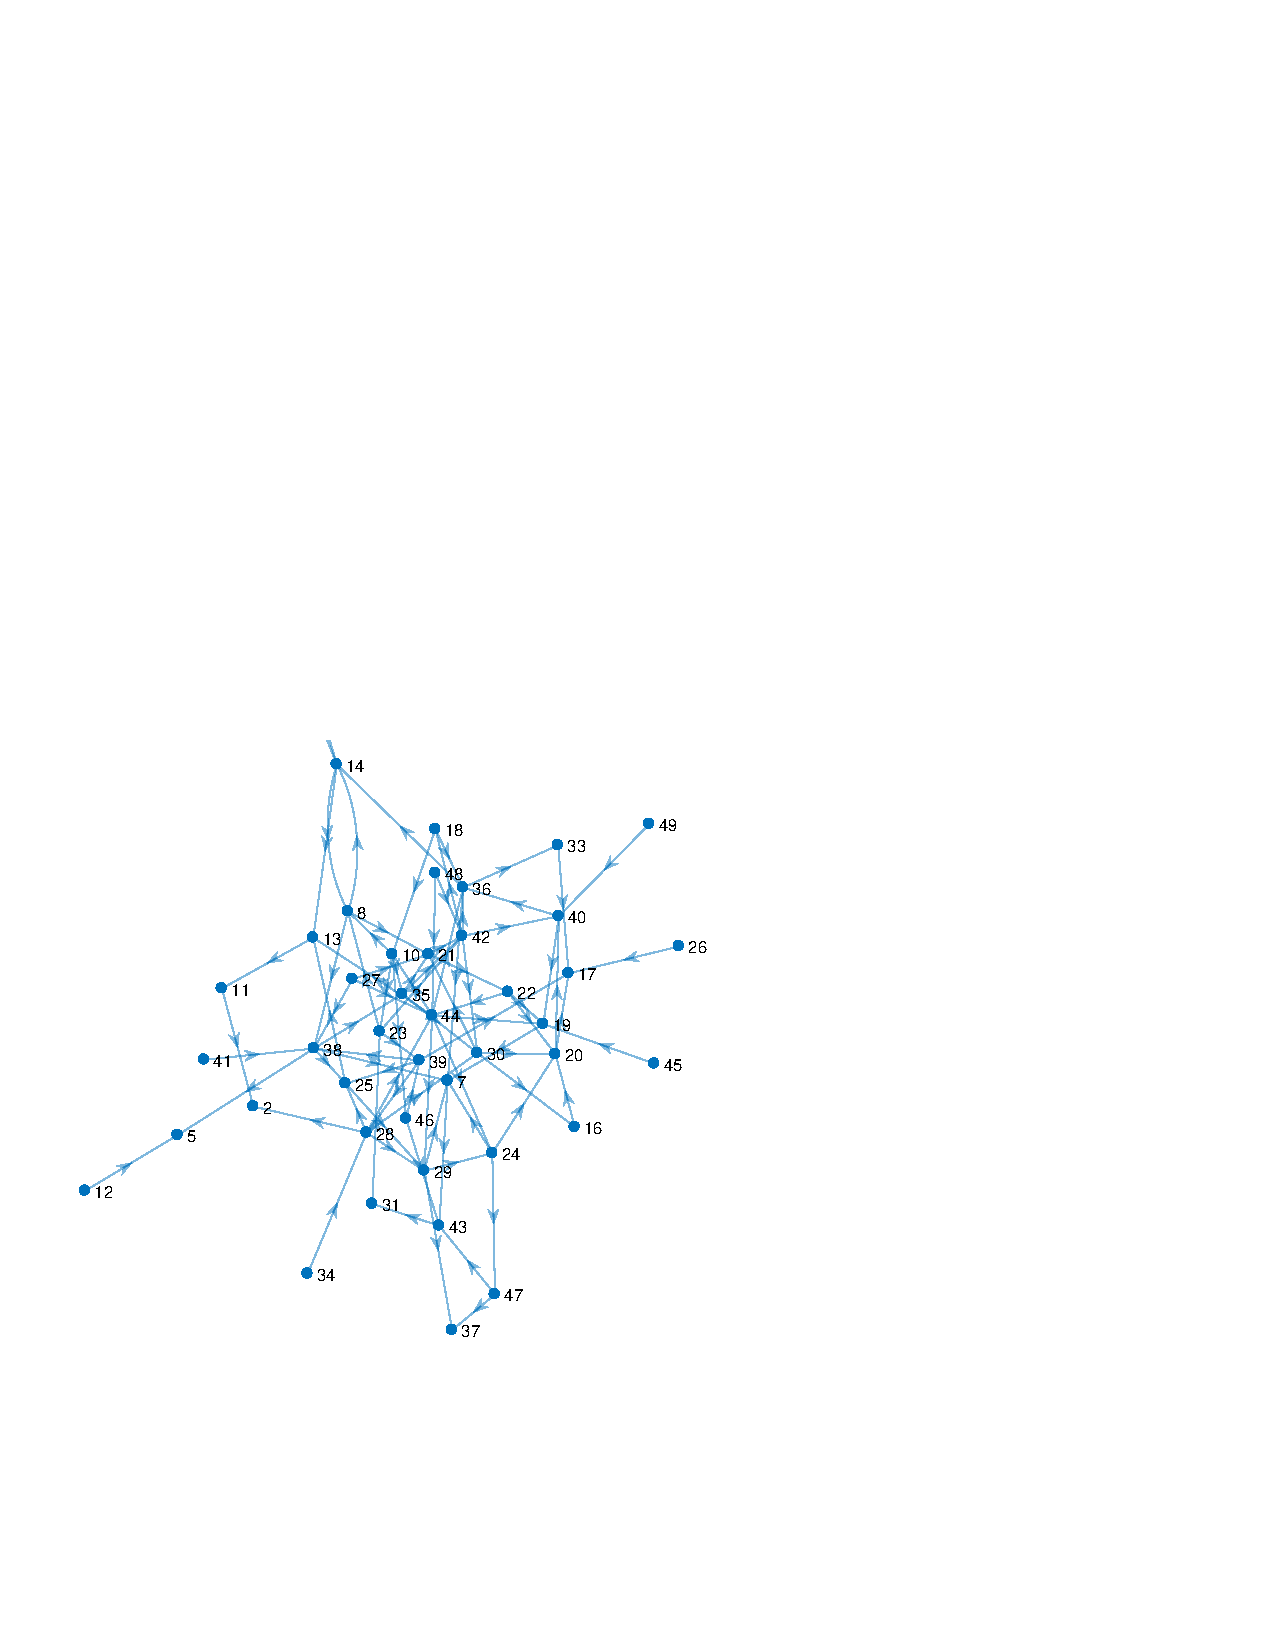
\includegraphics[width=0.8\linewidth]{dag}
%\caption{A Directed Acyclic Graph of the Running AUTOSAR Software Application, Runnables = 50, Paths = 35, Activation Patterns shown in Table \ref{tbl_requirements}.}
%\label{fig_application}
%\end{figure}
%\begin{center}
%\small
%\begin{minipage}{.5\textwidth}%
%\centering
%\begin{tabular}{@{}p{0.25cm}lll@{}}
%\toprule
%C& $r_i$ & $(e_{r_im_1}, e_{r_im_2}, e_{r_im_3})$ & $period$\\ \midrule
%\multirow{4}{4em}{c1} 
%&$r_1$ & (0.030, 0.060, 0.090) & 1\\
%&$r_2$ & (0.041, 0.081, 0.122) & 2\\
%&$r_3$ & (0.083, 0.167, 0.250)  & 5\\ 
%&$r_4$ & (0.310, 0.620, 0.930) & 10 \\[0.3em]
%\hline
%\multirow{2}{4em}{c2} 
%&$r_1$ & (0.310, 0.620, 0.930) & 10\\
%&$r_2$ & (0.310, 0.620, 0.930) & 10\\
%&$r_3$ & (0.310, 0.620, 0.930)  & 10\\ 
%&$r_4$ & (0.310, 0.620, 0.930) & 10 \\[0.3em]
%\hline
%\multirow{2}{4em}{c3} 
%&$r_1$ & (0.310, 0.620, 0.930) & 10\\
%&$r_2$ & (0.291, 0.583, 0.874)) & 10\\
%&$r_3$ & (0.291, 0.583, 0.874)  & 20\\ 
%&$r_4$ & (0.291, 0.583, 0.874) & 20 \\[0.3em]
%\hline
%\multirow{2}{4em}{c4} 
%&$r_1$ & (0.291, 0.583, 0.874) & 20\\
%&$r_2$ & (0.291, 0.583, 0.874)) & 10\\
%&$r_3$ & (0.291, 0.583, 0.874)  & 20\\ 
%&$r_4$ & (0.093, 0.186, 0.279) & 50 \\[0.3em]
%\hline
%\multirow{2}{4em}{c5} 
%&$r_1$ & (0.420, 0.841, 1.261) & 100\\
%&$r_2$ & (0.420, 0.841, 1.261)) & 100\\
%&$r_3$ & (0.420, 0.841, 1.261)  & 100\\ 
%&$r_4$ & (0.420, 0.841, 1.261) & 100 \\[0.3em]
%\bottomrule
%\end{tabular}
%\captionof{table}{Specification of Components.}
%\label{tbl_comps_config}
%\end{minipage}~
%\begin{minipage}{.45\textwidth}
%\begin{center}
%    \begin{tabular}{@{}lll@{}}
%    \toprule
%    Activation, $AP$ & Share & Time, ms \\ \midrule
%    $\tau_1$ & 50  & 50\\
%    $\tau_1\rightarrow\tau_2$ & 20  & 100\\
%    $\tau_1\rightarrow\tau_2\rightarrow\tau_3$ & 20  & 200\\
%    $\tau_1\rightarrow\tau_2\rightarrow\tau_3\rightarrow\tau_4$ & 10  & 400\\
%    \bottomrule
%    \end{tabular}
%    \captionof{table}{Activation Patters of Cause-effect Chains, their Share and End-to-end Timing Requirements.}
%    \label{tbl_requirements}
%\end{center}
%\begin{center}
%    \begin{tabular}{@{}llll@{}}
%    \toprule
%    M  & $P_{idle}$& $P_{busy}$& $\lambda$ \\ \midrule
%    $m_1$ & 50.0& 140.0 &1.0E-3  \\
%    $m_2$ & 10.0& 100.0 &1.0E-4  \\
%    $m_3$ & 10.0& 140.0 &1 .0E-5 \\ \bottomrule
%    \end{tabular}
%    \captionof{table}{Computation Nodes Specification.}
%    \label{tbl_nodes_specification}
%\end{center}
%\end{minipage}
%\end{center}

In the next section, we discuss our proposed method to address the considered optimization problem. 
